\section{Data cleaning and preprocessing}\label{sec:cleaning}
Cleaning is in \nolinkurl{src/weather/data/clean.py}. Every count below is written to
\nolinkurl{reports/metrics/clean_report.json} and logged to MLflow.

\paragraph{Schema.} The seven imperial duplicates (\textdegree F, mph, inches, miles) are dropped.
The pollutant columns are renamed (\texttt{aq\_pm25}, \dots), \texttt{last\_updated} is parsed to a timestamp,
and the snapshot's \emph{local clock hour} is kept as a covariate (Section~\ref{sec:hour}).

\paragraph{Coverage and duplicates.} 71 of the 268 location strings appear on fewer than 365 days
(3\,790 rows). They are one-off or mis-named entries and are removed, which leaves \textbf{197 capitals}.
Countries reported under translated names (e.g.\ Portuguese \emph{Polônia}, plus Cyrillic and Chinese spellings) are mapped back to
the canonical name each location uses most often. Continents come from \texttt{pycountry-convert} plus a
small override table. 385 same-day duplicate snapshots are collapsed, keeping the latest one.
Some locations are \emph{geocoding homonyms} (e.g.\ ``Yaren'' in Türkiye, ``Bogot'' in Bulgaria). Their
coordinates match the listed country, so their readings are valid weather for those coordinates and they are kept.

\paragraph{Physically invalid values.} Values outside plausible surface ranges become missing.
Examples are pressure of 3\,006\,mb, wind of 2\,963\,kph, and the sentinel $-9999$ in CO and SO$_2$.

\paragraph{Corrupted batches.} For each day we take the median, across all cities, of the absolute
difference between a city's temperature and its centred 15-day rolling median. A normal day sits near 1\,\textdegree C. On
\textbf{17~August~2026} it jumps to 8.5\,\textdegree C: Riyadh reads 15.6\,\textdegree C and Bishkek
4\,\textdegree C in mid-August. That day's weather values (186 rows) are nulled and re-imputed
(Figure~\ref{fig:batch}).

\paragraph{Outliers.} Roughly symmetric variables (temperature, feels-like, wind, gust, pressure) are capped
at a per-city fence $[Q_1-3\,\mathrm{IQR},\,Q_3+3\,\mathrm{IQR}]$. Heavy-tailed variables (precipitation and the
pollutants) are capped at the global 99.9th percentile. Capping (winsorising) keeps the row and stores a
boolean flag, so these points can still be studied in Section~\ref{sec:anomaly}.
Visibility is left out of the fence because it is reported as exactly 10\,km most of the time ($\mathrm{IQR}=0$).

\paragraph{Missing values.} Within each city, gaps are filled by time interpolation (up to 3 days), then
by the city median. Categorical gaps take the city mode. The raw file has no empty cells; every missing
value comes from the checks above.

\paragraph{Normalisation.} A \texttt{StandardScaler} is fitted on the \emph{training window only} and
persisted (\nolinkurl{models/scaler.joblib}). It is applied inside the linear model's pipeline. Anomaly
detection uses a \emph{city-local} standardisation instead (Section~\ref{sec:anomaly}).

\begin{figure}[H]\centering
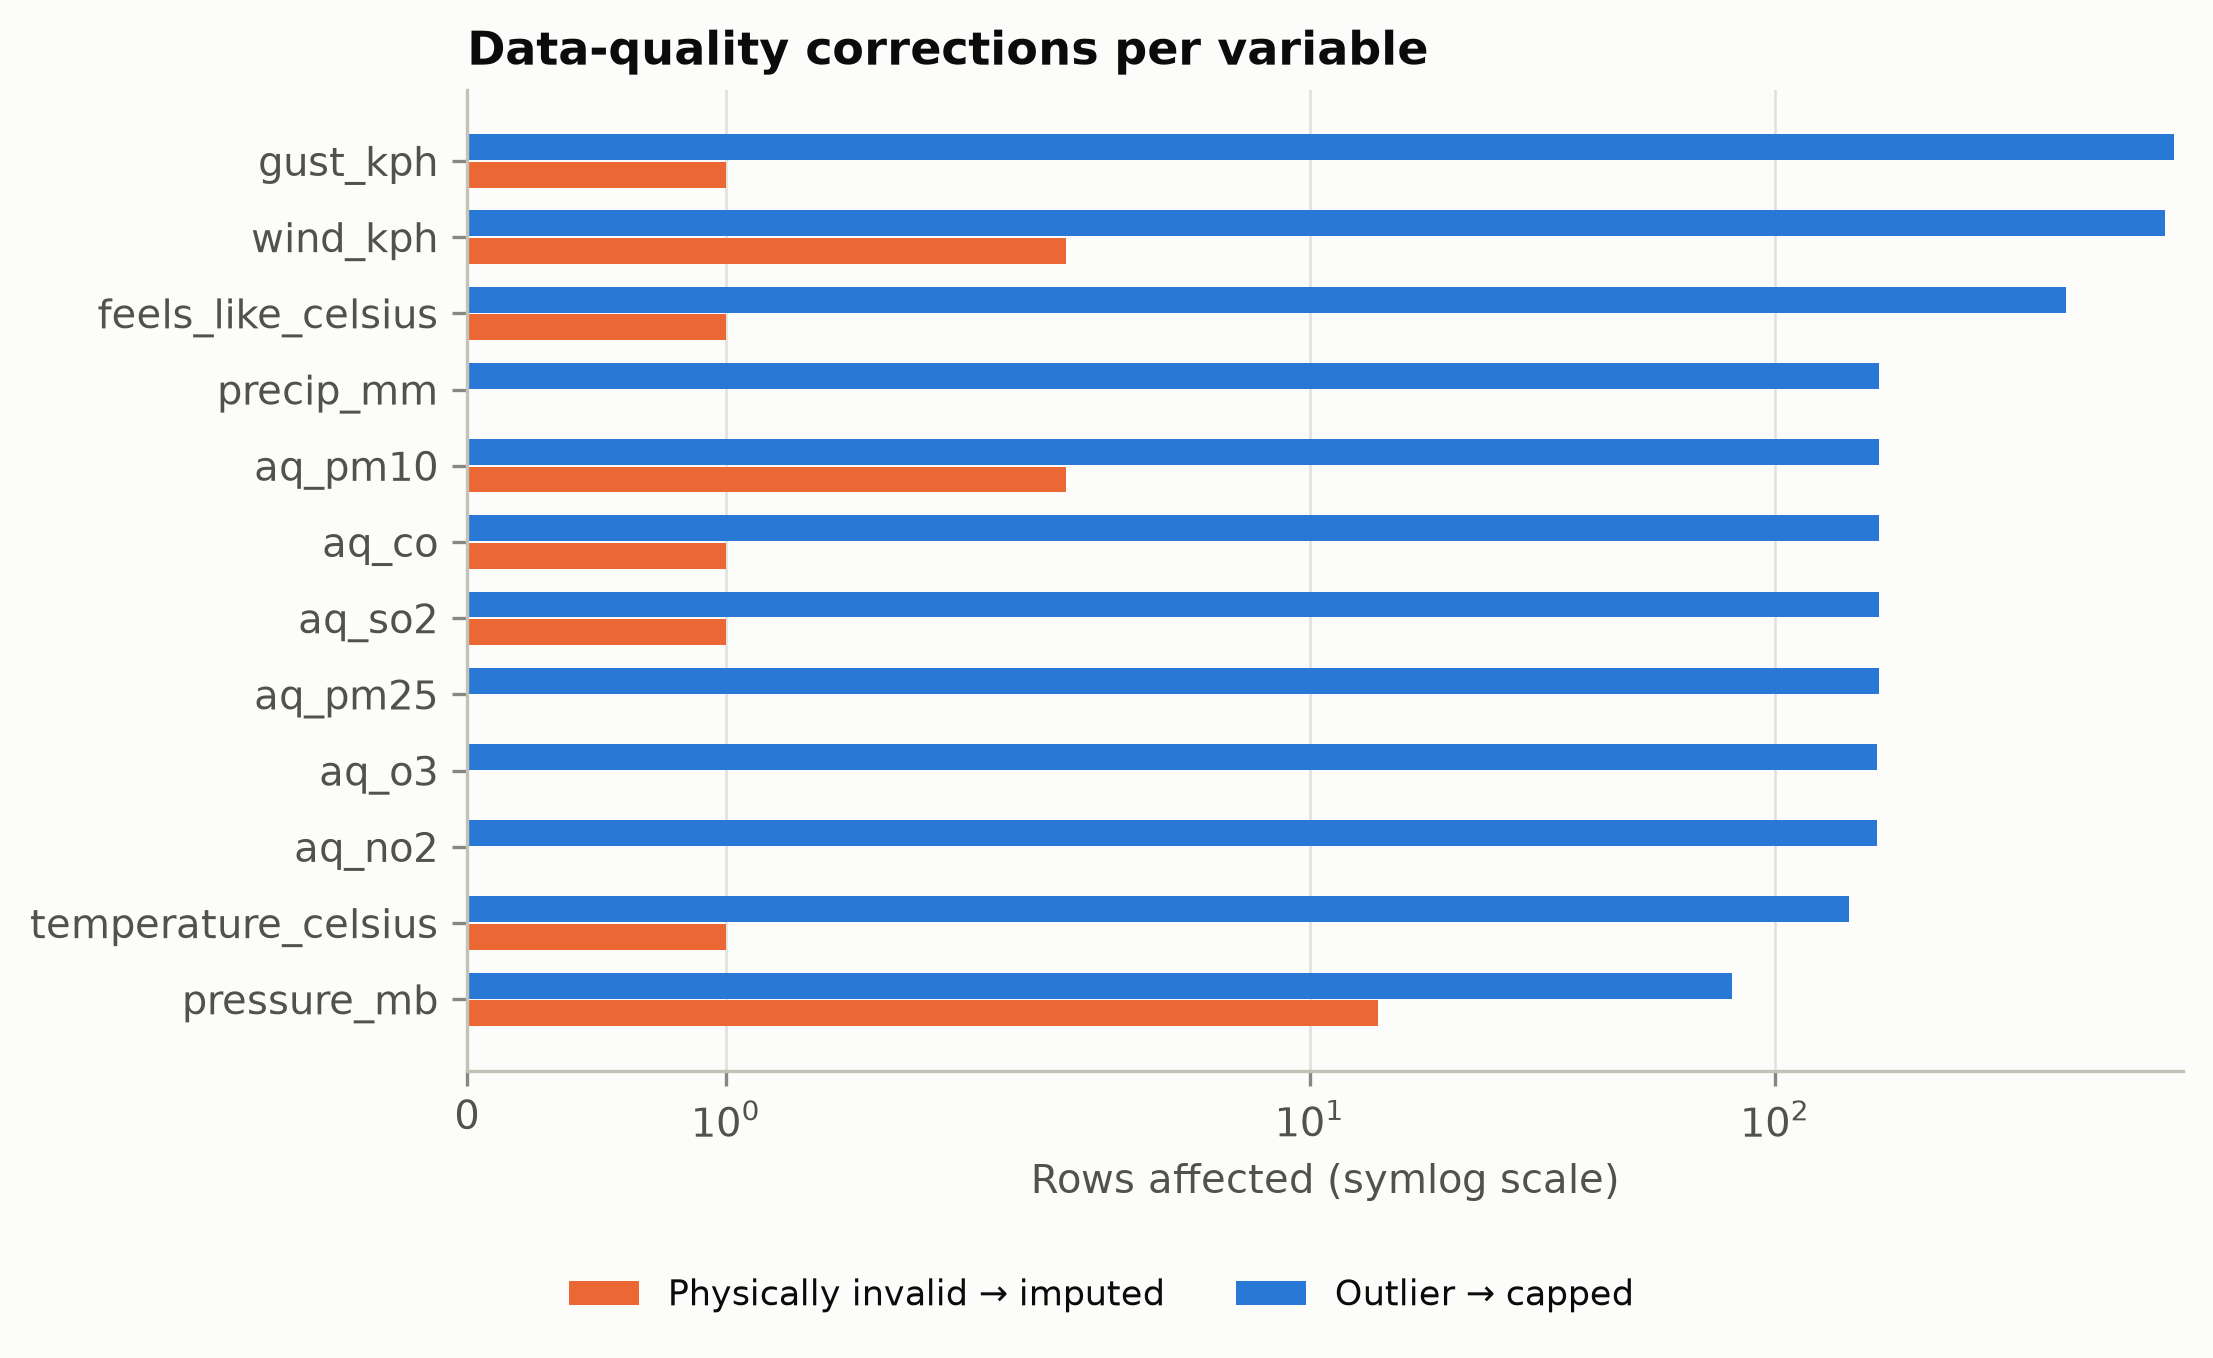
\includegraphics[width=0.75\linewidth]{eda/cleaning_corrections.png}
\caption{Rows corrected per variable: physically invalid values (imputed) and outliers (capped).}
\end{figure}

\paragraph{Feature engineering.} The cleaned data is put on a regular daily grid per city. Features use only
information available at day $t$:
\begin{itemize}
  \item today's temperature and its lags at 1, 2, 3, 7 and 14 days;
  \item rolling means and standard deviations over 3, 7 and 14 days, and the day-on-day difference;
  \item today's humidity, pressure, wind, gust, cloud, precipitation, UV, visibility and feels-like, plus
        changes in humidity and pressure;
  \item annual harmonics of the target date, also in a hemisphere-aware version;
  \item diurnal harmonics of the snapshot hour;
  \item latitude, longitude, $|$latitude$|$ and continent.
\end{itemize}
The target is temperature at $t+1$. The split is strictly by target date: the test window is the last
60 days (15~Aug--13~Oct~2026, 11\,213 rows), validation is the 60 days before it (11\,220 rows), and training is
everything earlier (142\,674 rows).
